\documentclass[a4paper]{article}
\usepackage[danish]{babel}
\usepackage[utf8]{inputenc}
\usepackage[]{graphicx}
\usepackage{verbatim}
\setcounter{tocdepth}{2}

\begin{document}

\thispagestyle{empty}
\begin{center}        % Sentrerer teksten
  %Tittel
  \vspace{5mm}          % Vertikalt mellomrom
  \LARGE
  \textbf{Procesanalyse} \\
  \Large
  \vspace{5mm}
  \textbf{ } \\
  \vspace{5mm}
  %Forfatter
  \large
  \textbf{Gruppe A215} \\
  %Avdeling for mekanikk
  \vspace{10mm}
  \Large
  {\bf{\textsl{ }}} \\
   \vspace{2mm}
  %%%%%%%OLD%%%%%%{\bf{\textsl{CANDIDATUS SCIENTIARUM}}} \\
  {\bf{\textsl{}}} \\
  \vspace{5mm}
  {\large \textsl {}}\\
  
  
  \vspace{10mm}
  \centerline{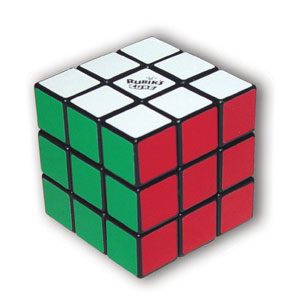
\includegraphics[width=4cm,height=4cm]{../rapport/input/pics/rubiksCube}}
  \vspace{5mm}
  % \textsl{Mechanics Division, Department of Mathematics} \\
  \textsl{} \\
  \textsl{} \\
  %Maaned, aar
  \vspace{10mm}
  \large
  \textsl{For\aa{}r 2010} \\
  \vspace{5mm}
  \normalsize
  % \textsl{Avdeling for mekanikk, Matematisk institutt} \\
  \textsl{} \\
  \textsl{} \\
\end{center}

\ \pagebreak{}
\tableofcontents{}
\ \pagebreak{}
\section{Projektplanl\ae{}gning}
Her gennemg\aa{}es essentielle projektplanl\ae{}gnings elementer. 

\subsection{Emnevalg}
I gruppen har der v\ae{}ret bred enighed om valg af emne. Retningen p\aa{} det emne var dog noget sv\ae{}rere at v\ae{}lge, men vi n\aa{}ede til en enighed hvor alle var tilfredse. 
Den endelige retning p\aa{} projekt blev f\o{}rst definitivt defineret meget sent i projektet.
Dette skyldtes at vi ikke fik lavet en grundig problemanalyse i starten af projektet.

Dette kan forbedres til P3 ved at lave en grundig problemanalyse i starten af projekt perioden. 

\begin{figure}[htbp]
\begin{center}
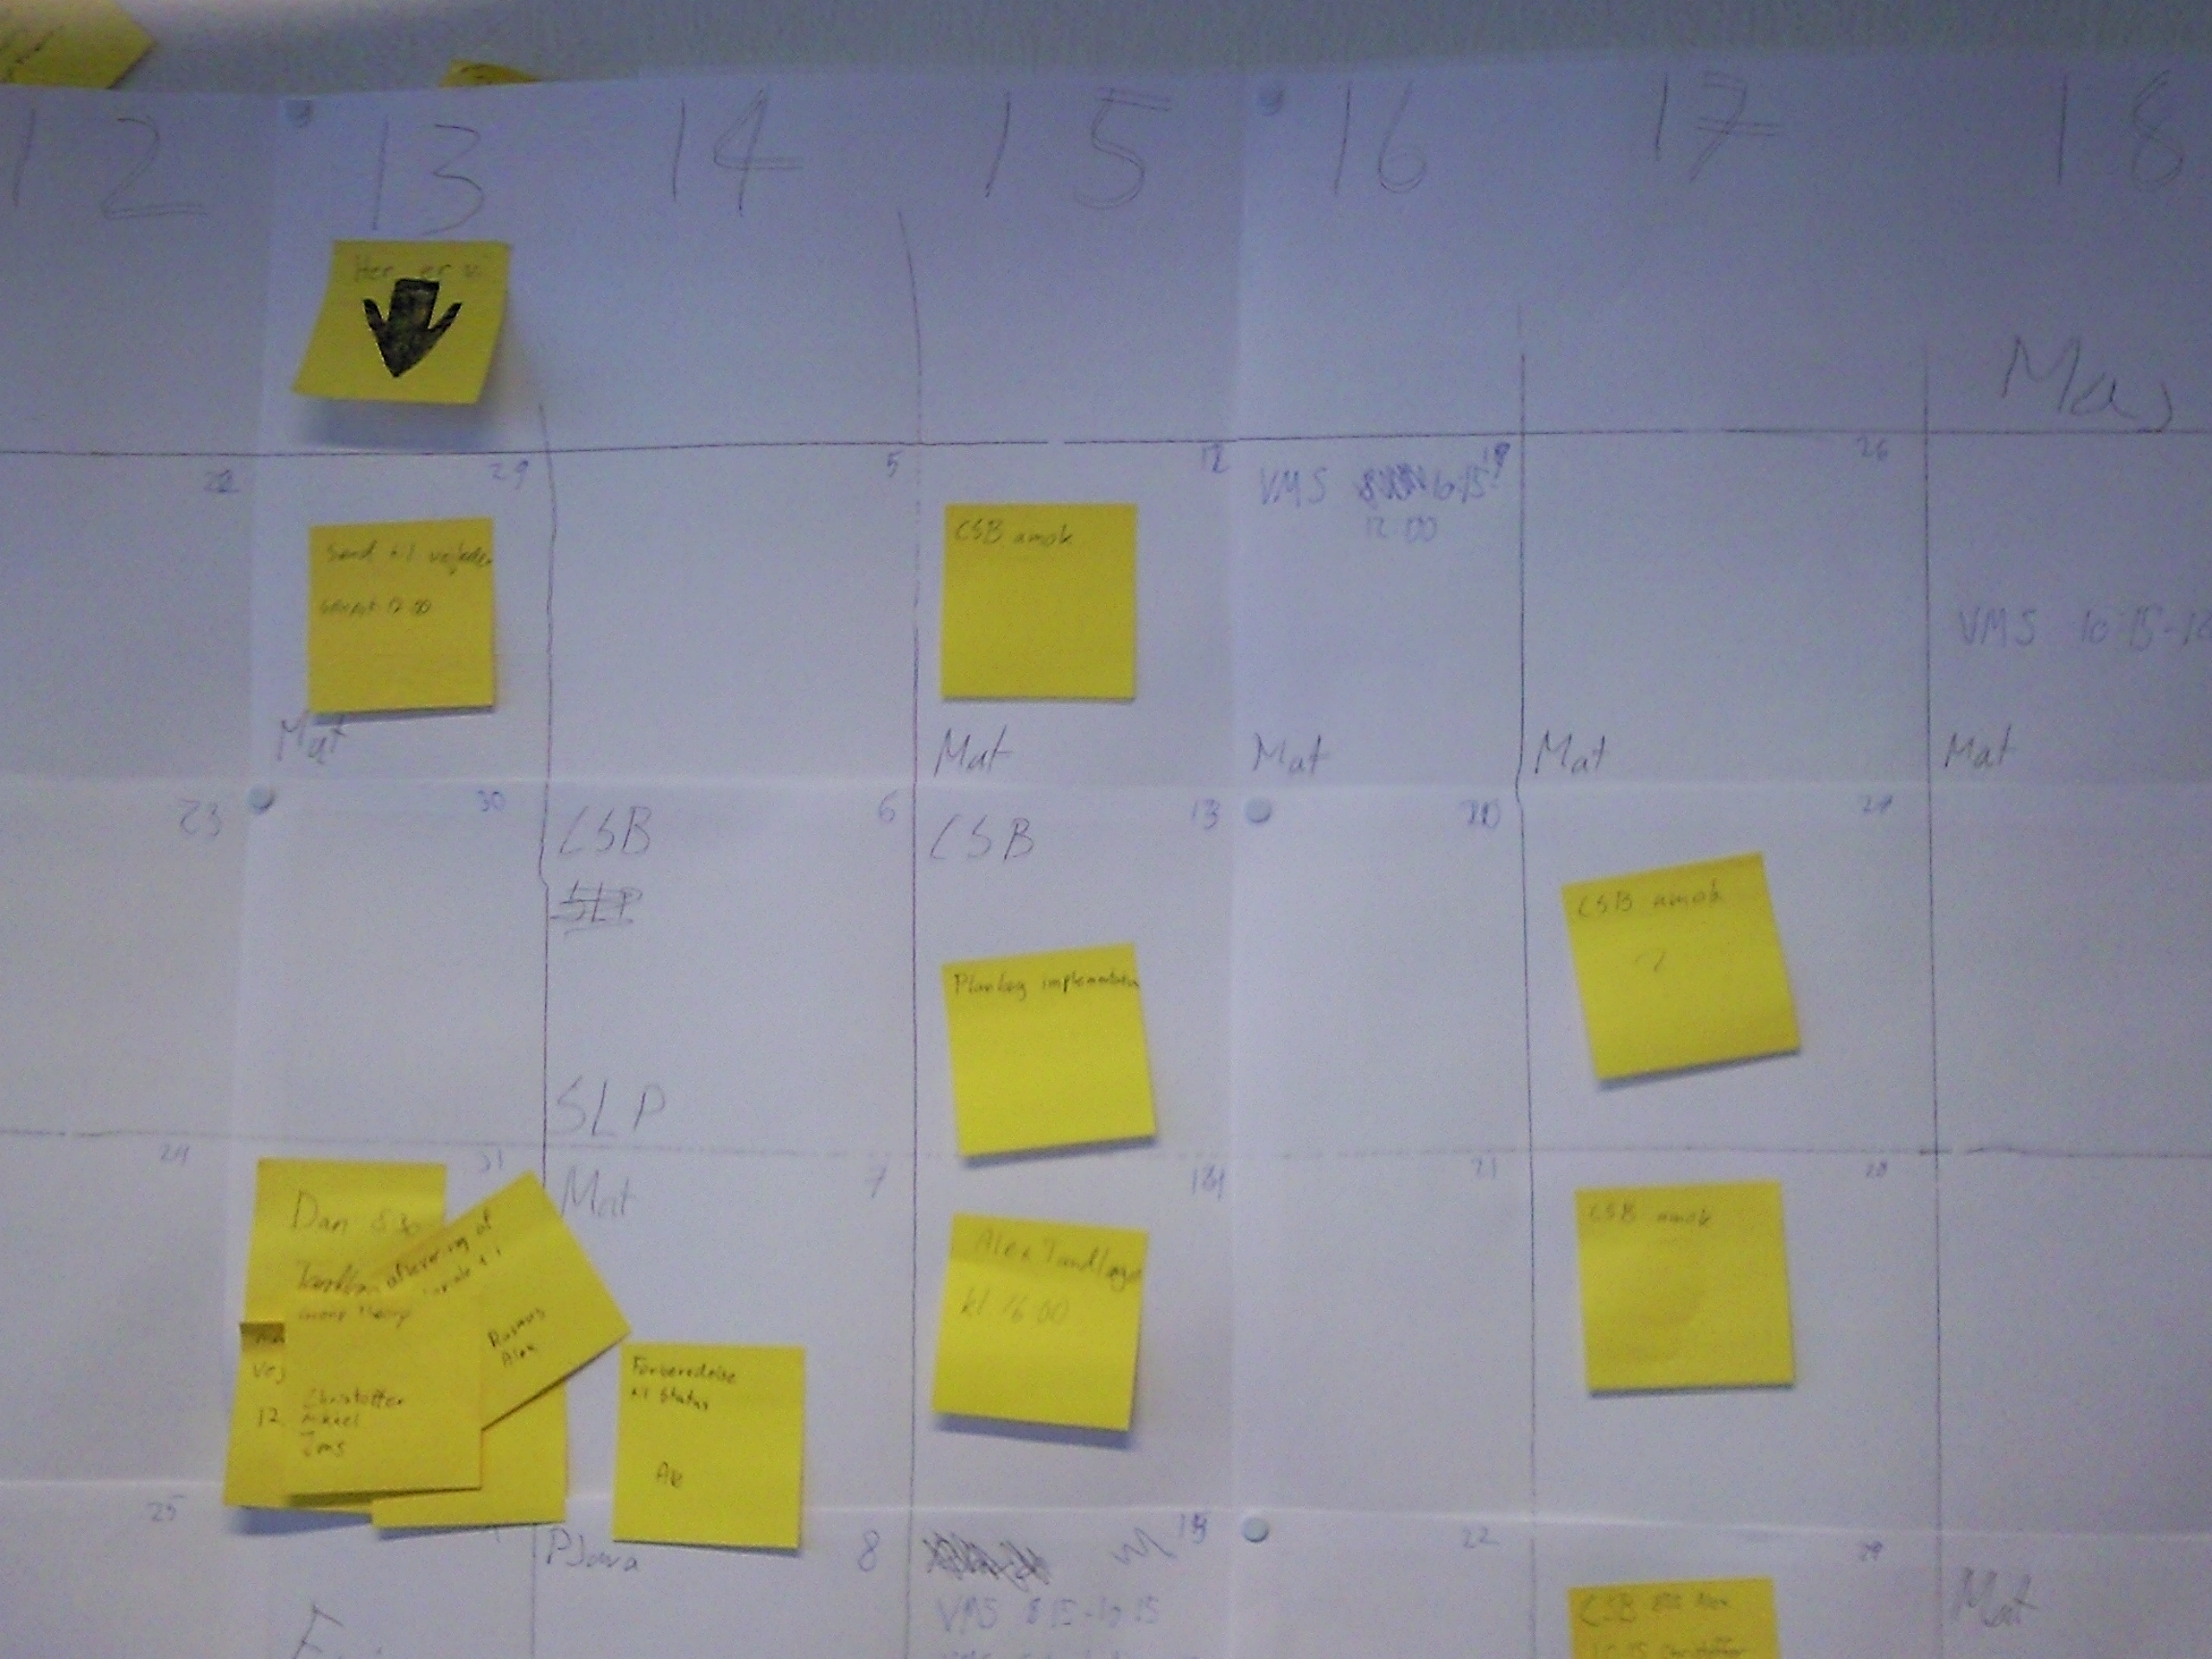
\includegraphics[width=\textwidth]{Billede0075.jpg}
\caption{default}
\label{default}
\end{center}
\end{figure}


\subsection{Tidstyring}
Til at administrere projektets arbejdsgang og tidsplan har vi anvendt en v\ae{}g kalender(see billede \ref{}), der fungerede b\aa{}de som opgavestyring og tidstyring. 

Kalenderen blev anvendt til at holde styr p\aa{} vores fastsatte deadlines. Hver opgave fik en post-it og blev opsat p\aa{} den dag hvor opgaven har deadline. Dette gav en stor fleksibilitet hvis opgavens omfang var fejlvurderet og den p\aa{}kr\ae{}vede tid til l\o{}sningen var st\o{}rre end f\o{}rst antaget, kunne post-it flyttes til en ny dato. 
 
I gennemretnings perioder virkede kalenderen dog ikke hensigtsm\ae{}sigt og vi anvendte tavler til styring af hvilke rapport elementer der blev retter af hvem. 
Kalenderen fungerede hensigtsm\ae{}ssigt og gav et l\o{}bende overblik over hvor i projektet vi stod og hvordan vi er med i forhold til deadlines. 

Til senere projekter kan et lignende system anvendes. Evt. en digitaliseret version da vores version optog meget v\ae{}g plads og en digitaliseret version kan tilg\aa{}s hjemmefra. 

\subsection{Projektstyring}
I gruppen valgte vi en flad demokratisk styringsform. Denne fungerede fint; alle emner og problemer blev diskuteret l\o{}bende. Dette var muligt da vi arbejdede stort set udelukkende i grupperummet og derved altid havde mulighed for at diskutere problemstillinger med hverandre. 

Vi har i projektet haft nogle roller, herunder; vejlederkontaktansvarlig, kontorkontaktansvarlig, trykkerikontaktansvarlig, kasserer, referent. Disse roller er delvist udefineret og nogle har v\ae{}ret skiftende roller.

Til P3 kunne der eksperimenteres med en defineret skiftende lederrolle for at opn\aa{} nogle lederkompetencer til alle gruppens medlemmer. 







\pagebreak
\section{Gruppesamarbejde}
Inden vi begyndte selve vores arbejdsproces diskuterede vi vores forventninger til hinanden. Vi havde generelt et h\o{}jt ambitionsniveau til vores rapport. 
Vi diskuterede hvad der kunne virke motiverende og demotiverende. Vi kom frem til at hvis der var nogen, der ikke arbejdede i et et tidsrum, hvor der var skulle arbejdes, kunne det virke demotiverende.
Derfor besluttede vi at vi i gruppen at alle skulle arbejde og holde pause p\aa{} samme tid. Dette udm\o{}ntede sig i at man kunne n\ae{}vne at man havde brug for en pause, hvorefter alle holdt pause. 
P\aa{} den m\aa{}de blev tid til arbejde og tid til pause direkte adskildt.


Vi startede projektprocessen med at udarbejde en samarbejdsaftale for gruppen. Mange af punkterne er blevet overholdt, men andre af punkterne er blevet glemt. 
Grunden til at nogle punkter ikke er blevet overholdt, er at arbejdsprocessen har g\aa{}et godt uden nogle enkelte af de v\ae{}rkt\o{}jer samarbejdsaftalen tilb\o{}d.


Vi har ikke holdt organiserede m\o{}der i gruppen. Vi har kun holdt m\o{}der n\aa{}r det virkede n\o{}dvendigt i gruppen. 
N\aa{}r et gruppemedlem f\o{}lte, at der var noget der kr\ae{}vende en diskussion, blev gruppen bedt om at lukke deres sk\ae{}rme ned og deltage i diskussionen. 
Diskussionen har v\ae{}ret fri; der har alts\aa{} ikke v\ae{}ret en m\o{}deleder eller ordstyrer.
Frekvensen af disse m\o{}der har v\ae{}ret svingende, da deres n\o{}dvendighed ikke har v\ae{}ret s\aa{} stor.


If\o{}lge vores samarbejdsaftale var der m\o{}depligt for gruppens medlemmmer alle hverdage fra kl. 08.15 til 15.00. 
Dette blev hovedsageligt overholdt, der var dog nogle gruppemedlemmer, der m\o{}dte for sent om morgenen. 
Dette f\o{}rte til en straffeordning, hvor det medlem, der m\o{}dte for sent skulle give kage til gruppen. 


Al gruppearbejde har foreg\aa{}et i grupperummet. Dette har medf\o{}rt at problemer hurtigt kunne im\o{}deg\aa{}es. 
Hovedsageligt deltog alle gruppemedlemmer i disse diskussioner.
Hvis et gruppemedlem har f\o{}lt sig umotiveret er dette blevet diskuteret og \aa{}rsagen til den manglende motivation blevet kortlagt, s\aa{} arbejdet kunne forts\ae{}tte.
Hvis hele gruppen har f\o{}lt sig umotiveret blev arbejdet sat p\aa{} stand-by, og der blev holdt en pause, hvor vi eksempelvis har spillet et computerspil sammen, eller s\aa{} tog vi fri og fortsatte arbejdet den f\o{}lgende dag.
Manglende motivation har dog ikke v\ae{}ret et seri\o{}st problem, og arbejdsprocessen har hovedsageligt forl\o{}bet efter planen.


Vi har i gruppen fordelt de forskellige emner, der skulle skrives om efter interesse; St\o{}rrelsen af emnerne er blevet vurderet og et passende antal gruppemedlemer blev sat p\aa{} det givne emne.

Arbejdet i gruppen har hovedsageligt foreg\aa{}et i mindre grupper p\aa{} omkring to eller tre gruppemedlemmer. Dette har generelt fungeret godt. 
Hvis der var problemer i en af de mindre grupper var det altid muligt at sp\o{}rge de andre gruppemedlemmer til r\aa{}ds, da alle var til stede i grupperummet.
Hvis et emne har v\ae{}ret st\o{}rre end f\o{}rst antaget, blev flere gruppemedlemmer flyttet til emnet, hvis det var muligt.

Hver dag blev tidspunktet for frokostpausen aftalt. I gruppen var der en madordning, hvor gruppemedlemmerne betalte et bestemt bel\o{}b hver uge, som der blev handlet ind for til frokost. 

Gruppearbejdet har gennemg\aa{}ende g\aa{}et godt. Vi har ikke g\aa{}et i st\aa{} i l\ae{}ngere tid, da vi altid har kunne sp\o{}rge hinanden til r\aa{}ds. Vores arbejdsprocess har v\ae{}ret produktiv, hvilket er en indikator for at den m\aa{}de, vi har arbejdet p\aa{}, har fungeret godt.

Selvom arbejdet i mindre grupper har fungeret godt, kunne man eksperimentere med at tildele arbejde hjemme. Dette kunne foreg\aa{} som et suplement til arbejde i gruppen, hvor nogle dage arbejdet foregik i grupperummet og andre dage bestod af arbejde hjemme.
Dette kunne muligvis effektivisere arbejde og undg\aa{} eventuelle gnidninger imellem gruppemedlemmer.

Til P3 ville det v\ae{}re en god ide at aftale sociale arrangementer p\aa{} forh\aa{}nd, i mods\ae{}tning til spontant, som det hovedsageligt er foreg\aa{}et i l\o{}bet af P2. 
Problemet med udelukkende spontane arrangementer er at, mange gruppemedlemmer ofte havde aftaler, og arrangementerne derfor ofte ikke blev til noget.
\pagebreak
\section{Samarbejde med vejlederne}
\label{H8R}

Vores samarbejde med vores hovedvejleder har v\ae{}ret rigtig godt. 
N\aa{}r vi har sendt noget materiale til ham, har vi f\aa{}et god og hurtig respons. 
Vi har n\ae{}sten haft m\o{}der hver uge med vores hovedvejleder, og der har altid v\ae{}ret god og
konstruktiv kritik. 
Vi har f\o{}lt at vores hovedvejleder har fulgt os igennem dette projekt og vist stor interesse for emnet, samt kommet med masser af forslag til forbedringer.

Vores samarbejde med vores bivejleder har ogs\aa{} fungeret godt, og hun har ogs\aa{} givet os god feedback. 
I starten havde vi mange m\o{}der med hende, men den sidste halvanden m\aa{}ned havde vi kun et m\o{}de, da vi kun skrev teori og implementation i denne periode.

N\aa{}r vi skulle sende arbejdsblade, som vi ville have respons p\aa{}, sendte vi dem til vejlederne 48 timer f\o{}r m\o{}det. Dette gav dem tid til at l\ae{}se dem igennem.

Et eksempel af et referat fra et af vores vejlederm\o{}der se sektion \ref{ref}

\subsection{Refleksion}
Vores samarbejde med vejlederne har generelt fungeret rigtig godt, og de har bidraget meget til projektets udformning. 
Nogle gange har vi v\ae{}ret frustrerede over nogle af de ting, de har sagt. 
Fx hvis det har v\ae{}ret st\o{}rre \ae{}ndringer i strukturen af rapporten. Andre gange har vi ikke forst\aa{}et pr\ae{}cist, hvad de
mente. 
Efter langt de fleste vejlederm\o{}der har vi dog siddet med f\o{}lelse af at have et godt overblik over rapporten og hvad der skulle ske efterf\o{}lgende. 
I slutfasen burde vi have holdt nogle flere m\o{}der med vores bivejleder, da hun havde en hel del \ae{}ndringer til det sidste m\o{}de. Vi burde have holdt det sidste m\o{} med vores bivejleder noget f\o{}r, og ikke tage for god vare, at hun sagde vores kontekstuelle del var fint halvanden m\aa{}ned inden afleverings datoen.


Afsnittet ``Samarbejde med vejledere'' i vores samarbejdsaftale, har vi ikke brugt, da vores samarbejde med vores vejledere har fungeret godt og de har altid kommet med konstruktiv kritik og vejledning. 
Vi fik ikke altid sendt vores arbejdsblade til vores vejledere i ordentlig tid, fordi vi var lidt pressede en gang imellem.

\subsection{Gode og d\aa{}rlige erfaringer}
Gode erfaringer, som vi vil bruge i P3:
\begin{itemize}
\item Vi pr\o{}vede altid at sende arbejdsbladene 48 timer inden m\o{}derne.
\end{itemize}
Ting, som vi vil g\o{}re anderledes i P3:
\begin{itemize}
\item Vi vil ikke tage det for god vare halvanden m\aa{}ned inden, n\aa{}r bivejleder siger at den kontekstuelle del er f\ae{}rdig, og vil f\o{}lge op p\aa{} det l\o{}bende ved at sende igen til bivejlederen.
\end{itemize}
\pagebreak
Hvordan har i arbejdet med læringsmål i gruppen?
Hvordan har i fulgt op på de læringsmål der blev defineret i gruppen? Har i nået målene?
Hvordan lærer du bedst, via individuelt arbejde – gruppediskussion – forelæsning etc.?
Hvordan har I brugt resultaterne af jeres individuelle læringsstilstest?
Hvilken læringsstrategi er efter jeres mening bedst i forbindelse med kurser? Hvorfor?
Hvordan hjælper I hinanden med at løse opgaver i kurserne?
Hvad gør I hvis I ikke forstår en forelæser eller det der står i bogen?
Hvilken læringsstrategi er efter jeres mening bedst i forbindelse med projektarbejdet? Hvorfor
Hvordan stimulerer og fremmer jeres vejledere jeres læreprocesser?


\section{Beskrivelse}
Da vi startede i vores P2 gruppe blev vi hurtige enige om nogen grundregler, og herefter fandt vi nogen l\ae{}ringsm\aa{}l som vi mente var realistiske at nå i løbet af projektforløbet.

Vi blev hurtigt enige om nogle forskellige læringsmål da vi begyndte med projektet, og de var som følger:

\begin{itemize}
\item L\ae{}r at l\o{}se Rubiks Cuben.
\item L\ae{}re at programmere i Java.
\item L\ae{}re  og forst\aa{} det bagved liggende matematik i Rubiks Terningen. 
\item L\ae{}e gruppe- og grafteori.
\end{itemize}

Vi har i gruppen arbejdet mod vores læringsmål, vi har ikke brugt det direkte som drivkræft for projektet, men vi har brugt dem til at definere retningen på vores projekt.
Flere af vores læringsmål har været essentielle punkter for indholdet af vores rapport, og derfor har vi kunnet arbejde med vores læringsmål samtidig med at vi har skrevet på vores projekt.

Vi har holdt et lille møde hvor vi har snakket lidt om hvordan det er gået med vores læringsmål. Da det er forskelligt hvordan folk lærer, og der er forskel på hvor meget folk går op i forskellige emner, så kan det være svært at lave en general bedømmelse. Vi har dog snakket lidt om hvordan det er gået med de enkelte læringsmål,

I skal beskrive jeres arbejdsprocesser i P1 så detaljeret som muligt indenfor de fire områder:
    •   Projektplanlægning
    •   Gruppesamarbejde
    •   Samarbejde med vejledere
    •   Læreprocesser
Beskrivelsen kan eksempelvis give et overblik over udviklingen i jeres arbejdsprocesser, ændringer
i processer undervejs, læringsmål, forventningsafklaringer i gruppen og med vejleder, aktiviteter til
opfølgning af målsætninger osv.


\section{Vurdering}

Når I er færdige med at beskrive hvad I gjorde, skal I vurdere hvordan det efter jeres mening gik.
Eksempelvis kan i komme ind på, hvordan i fulgte op på gruppens beslutninger og målsætninger og
i hvilket omfang jeres arbejdsprocesser indenfor de fire områder fungerede efter hensigten.


\section{Analyse}

Dernæst skal I analysere jeres arbejdsprocesser og få klarlagt hvorfor noget gik godt mens andet gik
dårligt. Med andre ord: Hvilke faktorer har indvirket på arbejdsprocesserne, og hvordan håndterede
i de udfordringer der opstod undervejs?


\section{Syntese}

Hvis jeres vurdering og analyse skal bidrage til at forbedre jeres evne til at håndtere det
problemorienterede og projektorganiserede gruppearbejde, skal I til slut konkretisere jeres
erfaringer i nogle ’Gode råd’ til jer selv og jeres medstuderende. En god måde at formulere sådanne
gode råd på er som en ’start-stop-fortsæt’-liste, dvs. en liste med følgende tre sektioner:
    •   Dette vil vi begynde at gøre i P2, som vi ikke gjorde i P1
    •   Dette vil vi ikke gøre i P2, som vi gjorde i P1
    •   Dette vil vi fortsætte med at gøre (gerne anderledes og bedre) i P2, som vi også gjorde i P1
Det er en god idé at tage ét af de fire områder ad gangen og gøre det færdigt. Husk hvad angår
strukturen at skelne klart mellem beskrivelse; vurdering og analyse og husk, at de ’Gode råd’ skal
være konkrete og operationelle, så de fører til reelle forbedringer i P2.

\pagebreak
\section{Referat}
\label{ref}
\begin{itemize}
	\item Advisor
	\item 
\end{itemize}

\subsection{Problem}
\begin{itemize}
	\item Mangler context, hvor er det henne?
	\item Kunne eventuelt skrive noget mere om Kociemba
	\item Noget konkret context
	\item Noget context med til det første punkt af problem statement, men man kan ikke se det med det samme
	\item Mere tydeligt i tops and tails om der er context, skriv det helt konkret
	\item Flyt Upper bound grafen op til ??? (ikke problem analysis, men måske chapter 4) og ændre lidt i det første punkt af problem statement
	\item Tag evt. en del af chap 9 med op
	\item Lav en problem analyse til at snævre indledeningen ind til problem statement.
	\item Hvad er formålet med projektet
	\item 
\end{itemize}


Nu snakker Heather
\begin{itemize}
	\item Parts of community, use groups instead
	\item God's algorithm, evt. italic
	\item Moving -> developping
	\item Noget galt til sidst i indledning
	\item Parts in limitations, what is it?
	\item Given -> chosen.
	\item page 7: both top and introduction, why? Maybe kill
	\item remove intro in chap 3
	\item page 8: hails - kill!! change to originate
	\item page 9: elaborate later -> below
	\item Similarities between magic cube and rubiks cube. State them!
	\item Permutations state similarities between and magic puzzle and rubiks cube -- The picture.
	\item page 11: Explain how Erno was inspired by the magic puzzle
	\item Cubie needs to be defined.
	\item page 14: using caps, watch it!
	\item p 19: 
\end{itemize}

\subsection{Theory}
\begin{itemize}
	\item p. 39: tail, use namely and ref to implementation part
	\item Perhaps use graph and group as context
	\item How has it been used earlier
	\item Add it to tops and tails
\end{itemize}

\subsection{Implementation}
\begin{itemize}
	\item Choices prior: change ref til prob. limit til at have det inline.
	\item Relate the tail to twist-wise community
	\item How does our choices relate to this community
	\item We position us in the technical community
	\item We make a contribution to the community in the form of analysis of the two algorithms
	\item Only refer back, don't tell the reader to read it.
\end{itemize}

Anders:
\begin{itemize}
	\item Statistics of Beginners: Elaborate, graphs, time
	\item Stats Kociemba: Eloborate, look at twist, change the header, describe $R^2$
\end{itemize}

\subsection{Epilogue}
\begin{itemize}
	\item What does the improvements do, Move to perspective/future work which is after conc
	\item Conclusion: Second question, is it important/interesting?
	\item Has anyone ever compared Kociamba to beginner's?
	\item In problem analysis descibe that we are interested in the two algos and maybe remove second question in problem statement.
	\item Upper and lower bound -- Define! -- should be done already.
	\item Refer back to the report, but no citations!
	\item Present the results from our tests, perhaps add to problem statement as well
	\item Maybe combine question 2 and 3
	\item Elaborate on the different algorithms there exists
\end{itemize}

\subsection{What to do}
See Heather's paper.


Remember to print the presentation and give it at the exam

\end{document}

\end{document}